\documentclass{article}

\usepackage{booktabs}
\usepackage{tabularx}
\usepackage{hyperref}
\usepackage{color, colortbl}
\usepackage{graphicx,array}
\usepackage{enumitem}
\usepackage{multirow}
\definecolor{LightCyan}{rgb}{0.88,1,1}
\hypersetup{
    colorlinks=true,       % false: boxed links; true: colored links
    linkcolor=red,          % color of internal links (change box color with linkbordercolor)
    citecolor=green,        % color of links to bibliography
    filecolor=magenta,      % color of file links
    urlcolor=cyan           % color of external links
}

\title{Hazard Analysis\\\progname}

\author{\authname}

\date{}

%% Comments

\usepackage{color}

\newif\ifcomments\commentstrue %displays comments
%\newif\ifcomments\commentsfalse %so that comments do not display

\ifcomments
\newcommand{\authornote}[3]{\textcolor{#1}{[#3 ---#2]}}
\newcommand{\todo}[1]{\textcolor{red}{[TODO: #1]}}
\else
\newcommand{\authornote}[3]{}
\newcommand{\todo}[1]{}
\fi

\newcommand{\wss}[1]{\authornote{blue}{SS}{#1}} 
\newcommand{\plt}[1]{\authornote{magenta}{TPLT}{#1}} %For explanation of the template
\newcommand{\an}[1]{\authornote{cyan}{Author}{#1}}

%% Common Parts

\newcommand{\progname}{ProgName} % PUT YOUR PROGRAM NAME HERE
\newcommand{\authname}{Team \#, Team Name
\\ Student 1 name and macid
\\ Student 2 name and macid
\\ Student 3 name and macid
\\ Student 4 name and macid} % AUTHOR NAMES                  

\usepackage{hyperref}
    \hypersetup{colorlinks=true, linkcolor=blue, citecolor=blue, filecolor=blue,
                urlcolor=blue, unicode=false}
    \urlstyle{same}
                                


\begin{document}

\maketitle
\thispagestyle{empty}

~\newpage

\pagenumbering{roman}

\begin{table}[hp]
	\caption{Revision History} \label{TblRevisionHistory}
	\begin{tabularx}{\textwidth}{llX}
		\toprule
		\textbf{Date} & \textbf{Developer(s)} & \textbf{Change}        \\
		\midrule
		Date1         & Name(s)               & Description of changes \\
		Date2         & Name(s)               & Description of changes \\
		...           & ...                   & ...                    \\
		\bottomrule
	\end{tabularx}
\end{table}

~\newpage

\tableofcontents

~\newpage

\pagenumbering{arabic}

\wss{You are free to modify this template.}

\section{Introduction}

In today's society, technology and engineering solutions are simply expected to work. The multitude of complex engineering designs and systems created to meet the needs of the world are expected to be infallible in the eyes of the public. When failures do occur, society considers them it shocking. When these failures happen in engineering systems critical to an aspect of safety, health, or some other critical role, people can die. In many cases, these failures are predictable and preventable in the design phase. The causes of such failures are known as hazards.
\subsection{Purpose of Hazard Analysis}

It is therefore necessary for engineers to perform extensive and thorough assessments of the systems they design in the aim to elimate as many failures as reasonably possible. This is process is called hazard analysis.\\

More formally, hazard analysis is a step in the process to assess risk within an engineering system. Its aim is to identify and assess the potential conditions which may cause failure. These hazards can exist and cause failures alone, or in combination with other hazards or conditions. Once completed, a hazard analysis should provide a comprehensive assessment of the hazards within a system according to the system's components and boundaries, the assumptions critical in performing judgements regarding hazards and the scenarios they may occur in, and the requirements necessary to ensure that these hazards will be mitigated within the realm of reasonable possibility.

\section{Scope}

The purpose of this document is to perform this hazard analysis on the system to be designed by the Back End Developers. This document will first provide a description of the system boundaries and components of the system on an abstract level (both the hardware and software components), and then will list and justify the assumptions made in order to perform this hazard analysis. These assumptions will be kept to a minimum, in the hope to reduce the number of potentially overlooked hazards. The document will then describe the Failure Mode and Effect Analysis (FMEA) done by the team of the Back End Developers, and then detail the specific safety and security requirements that have been discovered in the process of performing the hazard analysis. The document will end with a roadmap describing the steps which will be taken in order to implement the novel discovered requirements, the timeline in which they will be implemented, and what considerations must be made regarding said requirements.

\section{System Boundaries and Components}
The system consists of several components that make up the entire system

\subsection{Battery/Power Management system}
This component facilitates stepping down/up the source voltage from the battery to the necessary values required by different parts of the device. Moreover, it consists of a 										charge protection circuit for battery protection (Over-voltage and Discharge). Finally present is a battery level indicator that will generate an alert should the battery life fall below a certain threshold.

\subsection{Sensor Array system}
This component represents all the various sensors that will be used to collect the state information about the user. Also consists of various filters to facilitate smooth and accurate data collection.

\subsection{Prompt generation system}
This component handles  all prompt generation, from the detection of when a prompt occurs, to its specific creation and finally its display on the screen.

\subsection{Display System}
This system manages all functionality of the device's display, such as prompt display, showing basic user feedback such as date, time, temperature, etc.

\subsection{Data Storage system}
This system handles all logging and storage of data collected by both the sensor array and the prompt generator. Data is stored along with an indication of which system it came from and all prompts will be 				stored with the data and time of entry.

\subsection{Device Manager}
This system handles all connection and communication between the device and the host software.

\subsection{Error Handler - Hardware}
This component constantly checks the states of every system present and ensures that if any of them fail or return an error, an alert is generated. Moreover the system will also try to fix the problem 					wherever possible.

\subsection{Error Handler - Software}
This component monitors the state of the host software and will attempt to solve any errors that arise and will alert the user should the attempts fail.

\subsection{Host Software}
This system is the primary interface for the researchers to analyze the data collected by the device. It consists of several features that allows the researcher to set different
thresholds for activity tracking, calibrate all the sensors, update and create new records for participants, and finally interact with the data stored on the device.

\subsection{Calibration}
This system allows researchers to calibrate the sensors on the device , set and modify the different thresholds for activity tracking and create new prompts.

\subsection{Records}
This system stores all information about users present in the study. Moreover it provides functionality for researchers to create new records for new users.

\subsection{Data View}
This is where all data stored on the device can be viewed/ analyzed by the researchers in a graphical manner. The system also contains some functionality for data sorting/parsing and statistical analysis.

\subsection{System Boundary Diagram}
\begin{figure}
	\begin{center}
		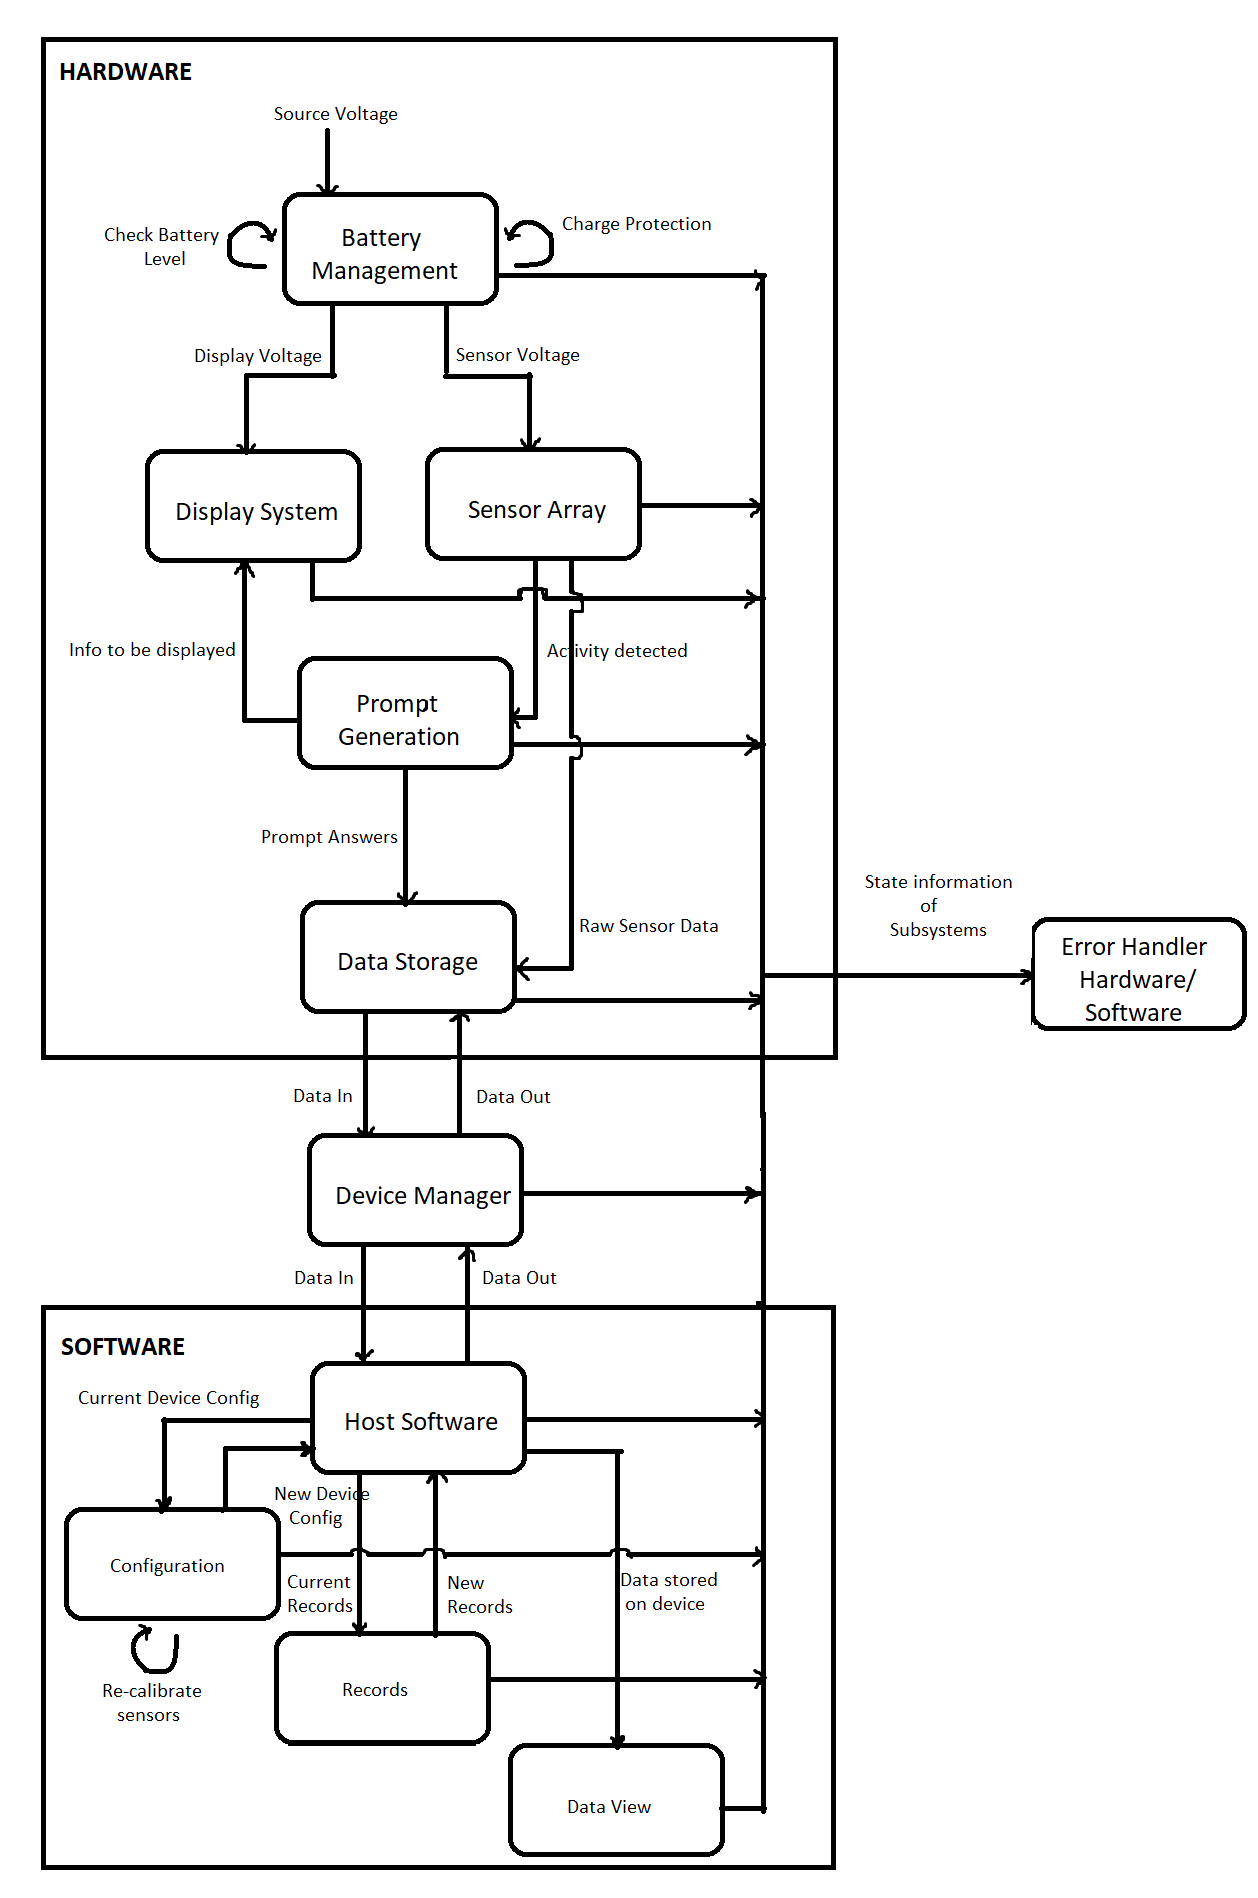
\includegraphics[width=1.0\textwidth]{SystemBoundaryDiagram}
		\caption{System Boundary Diagram}
		\label{Fig_SBD}
	\end{center}
\end{figure}
\pagebreak

\section{Critical Assumptions }

\begin{itemize}
	\item No wires will come loose during use.
	\item Batteries are pugged in correctly (the positive and negative ends are aligned as intended).
	\item All data are stored in the correct memory location.
	\item All subsystems work as intended.
	\item All off-the-shelf components work was intended.
\end{itemize}

\section{Failure Mode and Effect Analysis}
\begin{flushleft}
	\begin{tabular}{|p{6em}|p{5em}|p{5em}|p{5em}|p{5em}|p{9em}|}
		\hline
		\rowcolor{LightCyan}
		\textbf{Design Component} & \textbf{Failure Modes}                                        & \textbf{Causes of Failure} & \textbf{Effects of Failure} & \textbf{Detection} & \textbf{Recommended Action}\tabularnewline\hline
		%%%%%%%%%%%%%%%%%%%%%%%%%%%%%%%%%%%%%%%%%%%%%%%%%%%%%%%%%%%%%%%%%%%%%%%%%%%%%%%%%%%%%%%%%%%%%%%%%%%%%%%

		                          & Display not working                                           &
		\begin{minipage}[t]{\linewidth}
			\begin{itemize}[nosep, wide=0pt, leftmargin=*, after=\strut]
				\item Improper circuit connection
				\item Battery Level too low
				\item Code malfunction
				\item Physical damage to display
			\end{itemize}
		\end{minipage}

		                          & \begin{itemize}[nosep, wide=0pt, leftmargin=*, after=\strut]
			                            \item Users cannot answer prompts.
			                            \item Users cannot view any information on the display
		                            \end{itemize}

		                          & Display system returns an error code. Display Led is OFF
		                          & \begin{itemize}[nosep, wide=0pt, leftmargin=*, after=\strut]
			                            \item Users cannot answer prompts.
			                            \item Users cannot view any information on the display
			                            \item Check wiring and run a diagnostic on the display system
			                            \item Replace faulty hardware
		                            \end{itemize}
		\tabularnewline\cline{2-6}

		%%%%%%%%%%%%%%%%%%%%%%%%%%%%%%%%%%%%%%%%%%%%%%%%%%%%%%%%%%%%%%%%%%%%%%%%%%%%%%%%%%%%%%%%%%%%%%%%%%%%%%%

		\multirow{-8}{*}{\centering\rotatebox[origin=c]{90}{Display System}}

		                          & Incorrect information displayed
		                          & \begin{minipage}[t]{\linewidth}
			                            \begin{itemize}[nosep, wide=0pt, leftmargin=*, after=\strut]
				\item Display Driver faulty
				\item Improper interaction between Display system and Prompt generation
			\end{itemize}
		                            \end{minipage}

		                          & Users face unexpected outputs causing imporper use of device
		                          & Display system returns an error code.

		                          & \begin{minipage}[t]{\linewidth}
			                            \begin{itemize}[nosep, wide=0pt, leftmargin=*, after=\strut]
				\item Let Error Handler try to solve issue.
				\item Perform a manual overview of code.
				\item Perform a system reboot.
			\end{itemize}
		                            \end{minipage}  \tabularnewline\cline{1-6}
	\end{tabular}%\vspace{3mm}
	%%%%%%%%%%%%%%%%%%%%%%%%%%%%%%%%%%%%%%%%%%%%%%%%%%%%%%%%%%%%%%%%%%%%%%%%%%%%%%%%%%%%%%%%%%%%%%%%%%%%%%%


	\begin{tabular}{|p{6em}|p{5em}|p{5em}|p{5em}|p{5em}|p{9em}|}


		%%%%%%%%%%%%%%%%%%%%%%%%%%%%%%%%%%%%%%%%%%%%%%%%%%%%%%%%%%%%%%%%%%%%%%%%%%%%%%%%%%%%%%%%%%%%%%%%%%%%%%%

		\hline
		 & Prompt not generated                                                                   &
		\begin{minipage}[t]{\linewidth}
			\begin{itemize}[nosep, wide=0pt, leftmargin=*, after=\strut]
				\item Prompt generation code faulty
				\item System stuck in an idle state where no activity is detected.
			\end{itemize}
		\end{minipage}

		 &
		\begin{itemize}[nosep, wide=0pt, leftmargin=*, after=\strut]
			\item Display system will not produce an output.
			\item Users will be unable to provide feedback regarding activity
		\end{itemize}

		 & Prompt Generation system returns an error code.
		 & Let Error Handle try to solve the issue  \tabularnewline\cline{2-6}

		%%%%%%%%%%%%%%%%%%%%%%%%%%%%%%%%%%%%%%%%%%%%%%%%%%%%%%%%%%%%%%%%%%%%%%%%%%%%%%%%%%%%%%%%%%%%%%%%%%%%%%%

		\multirow{-8}{*}{\centering\rotatebox[origin=c]{90}{Prompt Generation System}}

		 & Incorrect Prompt Generated
		 & \begin{minipage}[t]{\linewidth}
			   \begin{itemize}[nosep, wide=0pt, leftmargin=*, after=\strut]
				\item Prompt generation code faulty
				\item Improper interaction between Prompt generation and Sensor Array
			\end{itemize}
		   \end{minipage}

		 & Prompt generated produces unexpected outputs causing imporper use of device
		 & Prompt Generation system returns an error code. Test prompt produces unexpeted outputs

		 & \begin{minipage}[t]{\linewidth}
			   \begin{itemize}[nosep, wide=0pt, leftmargin=*, after=\strut]
				\item Let Error Handler try to solve issue.
				\item Check System Array State
				\item Perform a system reboot.
			\end{itemize}
		   \end{minipage}  \tabularnewline\cline{1-6}
	\end{tabular}%\vspace{3mm}
	%%%%%%%%%%%%%%%%%%%%%%%%%%%%%%%%%%%%%%%%%%%%%%%%%%%%%%%%%%%%%%%%%%%%%%%%%%%%%%%%%%%%%%%%%%%%%%%%%%%%%%%

	\begin{tabular}{|p{6em}|p{7em}|p{5em}|p{5em}|p{5em}|p{9em}|}
		\hline
		 & \begin{minipage}[t]{\linewidth}
			   \begin{itemize}[nosep, wide=0pt, leftmargin=*, after=\strut]
				\item Heart rate not detected
				\item Surrounding pressure not being tracked
				\item No motion detected
			\end{itemize}
		   \end{minipage} &
		\begin{minipage}[t]{\linewidth}
			\begin{itemize}[nosep, wide=0pt, leftmargin=*, after=\strut]
				\item Device not worn properly
				\item Sensor breaks down, due to passing thresholds limits
				\item Device surface is dusty or contaminated
			\end{itemize}
		\end{minipage}
		 & EMA may not be triggered        & Software check to see if any sensor data is being collected &
		\begin{minipage}[t]{\linewidth}
			\begin{itemize}[nosep, wide=0pt, leftmargin=*, after=\strut]
				\item Ensure the device has been wrapped around properly for more accurate detection
				\item Reboot the system
				\item Let error handler try to solve the issue
			\end{itemize}
		\end{minipage}  \tabularnewline\cline{1-6}

		%
		\multirow{-16}{*}{\centering\rotatebox[origin=c]{90}{Sensor Array}}
		\multirow{16}{*}{\centering\rotatebox[origin=c]{90}{Battery management system}}
		 & Device not starting             & \begin{minipage}[t]{\linewidth}
			                                     \begin{itemize}[nosep, wide=0pt, leftmargin=*, after=\strut]
				\item Device is faulty
				\item Battery has died
				\item Device may have overheated
				\item Water may have damaged the battery
			\end{itemize}
		                                     \end{minipage}                             & Device is not turned on, resulting in no monitoring & Battery dead indicator appears when turning on the device &
		\begin{minipage}[t]{\linewidth}
			\begin{itemize}[nosep, wide=0pt, leftmargin=*, after=\strut]
				\item Charge the device
				\item Change batteries if needed
			\end{itemize}
		\end{minipage}  \tabularnewline\cline{1-6}
	\end{tabular}%\vspace{3mm}



	\begin{tabular}{|p{6em}|p{7em}|p{5em}|p{5em}|p{5em}|p{9em}|}
		%
		\hline
		 & Security Compromised                                     &
		\begin{minipage}[t]{\linewidth}
			\begin{itemize}[nosep, wide=0pt, leftmargin=*, after=\strut]
				\item Fail-open security check
				\item Error data improperly protected
				\item Malicious cyber attack
			\end{itemize}
		\end{minipage}
		 & Participant data will be made vulnerable to exploitation & Error handler returns strange or incomplete results & Device enters data-lockdown mode, preventing data from being accessed until security issue is resolved. \tabularnewline\cline{2-6}

		%
		\multirow{-8}{*}{\centering\rotatebox[origin=c]{90}{Error Handler}}
		 & Errors are strange or incomplete                         & \begin{minipage}[t]{\linewidth}
			                                                              \begin{itemize}[nosep, wide=0pt, leftmargin=*, after=\strut]
				\item Stack overflow
				\item Memory leak
				\item Error previously unaccounted for
			\end{itemize}
		                                                              \end{minipage}                     & Persons responsible for responding to errors will be unable to diagnose and address the underlying issue                           & Error comes in an unexpected form, or returns no value & \begin{minipage}[t]{\linewidth}
			                                                                                                                                                                                                                                                                                                 \begin{itemize}[nosep, wide=0pt, leftmargin=*, after=\strut]
				\item Use different channels to handle device logic and error handling
				\item Ensure that strange errors either return as Optional or Empty List (i.e. any value but null)
			\end{itemize}
		                                                                                                                                                                                                                                                                                                 \end{minipage}  \tabularnewline\cline{1-6}
	\end{tabular}%\vspace{3mm}


	\begin{tabular}{|p{6em}|p{7em}|p{6em}|p{5em}|p{5em}|p{9em}|}
		\hline                                                                                                           &
		Data stored at wrong memory location                                                                             &
		\begin{minipage}[t]{\linewidth}
			\begin{itemize}[nosep, wide=0pt, leftmargin=*, after=\strut]
				\item Incorrect software commands
				\item Memory space doesn't exist (invalid memory selected)
				\item Insufficient memory space
				\item Physical damage to hardware memory chip
			\end{itemize}
		\end{minipage}                                                                                  &
		Lost and unsaved data                                                                                            &
		Set up error handler to check if each data point is successfully stored at the correct memory location each time &
		Replace faulty hardware or set up correct memory path
		\tabularnewline\cline{2-6}

		\multirow{-15}{*}{\centering\rotatebox[origin=c]{90}{Data Storage}}
		                                                                                                                 &
		Data Stored with incorrect type                                                                                  &
		\begin{minipage}[t]{\linewidth}
			\begin{itemize}[nosep, wide=0pt, leftmargin=*, after=\strut]
				\item Wrong data type used for storing data
			\end{itemize}
		\end{minipage}                                                                                  &
		Analysis program can't interpret data                                                                            &
		Failed data analysis                                                                                             &
		Convert data to correct type
		\tabularnewline\cline{1-6}
		\multirow{15}{*}{\centering\rotatebox[origin=c]{90}{Device manager}}
		                                                                                                                 &
		Unable to establish connection                                                                                   &
		\begin{minipage}[t]{\linewidth}
			\begin{itemize}[nosep, wide=0pt, leftmargin=*, after=\strut]
				\item Loose wires
				\item Incorrect communication protocol
				\item Incorrect parameters for serial packets (size, format, etc.)
			\end{itemize}
		\end{minipage}                                                                                  &
		\begin{minipage}[t]{\linewidth}
			\begin{itemize}[nosep, wide=0pt, leftmargin=*, after=\strut]
				\item Data can't be transferred between hardware and software
				\item Lost data
			\end{itemize}
		\end{minipage}                                                                                  &
		\begin{minipage}[t]{\linewidth}
			\begin{itemize}[nosep, wide=0pt, leftmargin=*, after=\strut]
				\item Check list of connected devices on device manager
				\item Visual inspection of wiring and circuitry
				\item Attach an error detection LED on the device
			\end{itemize}
		\end{minipage}                                                                                  &
		\begin{minipage}[t]{\linewidth}
			\begin{itemize}[nosep, wide=0pt, leftmargin=*, after=\strut]
				\item Make sure all necessary connections are made
				\item Reboot device
				\item Restart host software
			\end{itemize}
		\end{minipage}
		\tabularnewline\cline{1-6}
	\end{tabular}



	\begin{tabular}{|m{6em}|m{5em}|m{5em}|m{5em}|m{5em}|m{9em}|}
		\hline
		%%%%%%%%%%%%%%%%%%%%%%%%%%%%%%%%%%%%%%%%%%%%%%%%%%%%%%%%%%%%%%%%%%%%%%%%%%%%%%%%%%%%%%%%%%%%%%%%%%%%%%%

		 & Records not created and deletion of records                             &
		\begin{minipage}[t]{\linewidth}
			\begin{itemize}[nosep, wide=0pt, leftmargin=*, after=\strut]
				\item Code that writes to database is faulty.
				\item	Connections between software systems are incorrect.
			\end{itemize}
		\end{minipage}

		 & \begin{itemize}[nosep, wide=0pt, leftmargin=*, after=\strut]
			   \item Present users lose data, new users cannot have data stored.
			   \item Time loss.
		   \end{itemize}

		 &
		\begin{itemize}[nosep, wide=0pt, leftmargin=*, after=\strut]
			\item Records system returns an error code using error checking.
			\item Database trigger for stagnant data.
		\end{itemize}

		 & Create redundant data sets and storage units, or cloud storage of data.
		\tabularnewline\cline{2-6}

		%%%%%%%%%%%%%%%%%%%%%%%%%%%%%%%%%%%%%%%%%%%%%%%%%%%%%%%%%%%%%%%%%%%%%%%%%%%%%%%%%%%%%%%%%%%%%%%%%%%%%%%

		\multirow{-8}{*}{\centering\rotatebox[origin=c]{90}{Records}}

		 & Corrupted records
		 & \begin{minipage}[t]{\linewidth}
			   \begin{itemize}[nosep, wide=0pt, leftmargin=*, after=\strut]
				\item Code is faulty.
				\item Database structure is faulty.
				\item Wrong datatype used for storing data.
			\end{itemize}
		   \end{minipage}

		 & Data stored for various users is unusable.
		 &
		\begin{minipage}[t]{\linewidth}
			\begin{itemize}[nosep, wide=0pt, leftmargin=*, after=\strut]
				\item Detect if data records are returning unusable values, e.g. NaN, Inf, 0, garbage values.
				\item View values stored in database to check for unexpected outputs.
			\end{itemize}
		\end{minipage}

		 & \begin{minipage}[t]{\linewidth}
			   \begin{itemize}[nosep, wide=0pt, leftmargin=*, after=\strut]
				\item Prevent users from accessing database.
				\item Ensure database is robust prior to deployment through testing.
			\end{itemize}
		   \end{minipage}  \tabularnewline\cline{1-6}
	\end{tabular}%\vspace{3mm}
	%%%%%%%%%%%%%%%%%%%%%%%%%%%%%%%%%%%%%%%%%%%%%%%%%%%%%%%%%%%%%%%%%%%%%%%%%%%%%%%%%%%%%%%%%%%%%%%%%%%%%%%




	\begin{tabular}{|m{6em}|m{5em}|m{5em}|m{5em}|m{5em}|m{9em}|}


		%%%%%%%%%%%%%%%%%%%%%%%%%%%%%%%%%%%%%%%%%%%%%%%%%%%%%%%%%%%%%%%%%%%%%%%%%%%%%%%%%%%%%%%%%%%%%%%%%%%%%%%

		\hline
		 & Data not visible                                                                  &
		\begin{minipage}[t]{\linewidth}
			\begin{itemize}[nosep, wide=0pt, leftmargin=*, after=\strut]
				\item Data collection failure.
				\item Poorly aggregated data.
				\item Incorrect software implementation.
				\item Statistical analysis of data is faulty.
			\end{itemize}
		\end{minipage}

		 & Information provided is not useful to researchers or participants.
		 & \begin{itemize}[nosep, wide=0pt, leftmargin=*, after=\strut]
			   \item Error handling to detect if the software is not performing as it should be.
			   \item Check error codes of device manager.
		   \end{itemize}

		 &
		\begin{itemize}[nosep, wide=0pt, leftmargin=*, after=\strut]
			\item Visual inspection to make sure device is working.
			\item Ensure database is robust prior to deployment through testing
		\end{itemize} \tabularnewline\cline{2-6}

		%%%%%%%%%%%%%%%%%%%%%%%%%%%%%%%%%%%%%%%%%%%%%%%%%%%%%%%%%%%%%%%%%%%%%%%%%%%%%%%%%%%%%%%%%%%%%%%%%%%%%%%

		\multirow{-8}{*}{\centering\rotatebox[origin=c]{90}{Data View}}

		 & Graphical data representation incorrect.
		 & \begin{minipage}[t]{\linewidth}
			   \begin{itemize}[nosep, wide=0pt, leftmargin=*, after=\strut]
				\item Improper communication with device manager.
				\item Device malfunction, no correct data.
			\end{itemize}
		   \end{minipage}

		 & Incorrect observations could be made based on the data.
		 & \begin{minipage}[t]{\linewidth}
			   \begin{itemize}[nosep, wide=0pt, leftmargin=*, after=\strut]
				\item Error handling to detect if the software is not performing as it should be.
				\item Check error codes of device manager
			\end{itemize}
		   \end{minipage}

		 & \begin{minipage}[t]{\linewidth}
			   \begin{itemize}[nosep, wide=0pt, leftmargin=*, after=\strut]
				\item Visual inspection to make sure device is working.
				\item Use error handler to solve issue.
			\end{itemize}
		   \end{minipage}  \tabularnewline\cline{1-6}
	\end{tabular}%\vspace{3mm}



	\begin{tabular}{|p{3em}|p{5em}|p{5em}|p{8em}|p{8em}|p{8em}|}
		\hline
		 & Calculation and floating point errors                                                                                                                      &
		\begin{minipage}[t]{\linewidth}
			\begin{itemize}[nosep, wide=0pt, leftmargin=*, after=\strut]
				\item Improper units used (metric vs Imperial)
				\item Rounding error
				\item Floating point conversion error
			\end{itemize}
		\end{minipage}

		 & \begin{itemize}[nosep, wide=0pt, leftmargin=*, after=\strut]
			   \item Wrong information can be reported if units are not consistent.
			   \item Rounding errors can carry forward through different formulas resulting in improper final results which can cause the data to be inaccurate.
			   \item Data calculated will be completely wrong due to binary overflow.
		   \end{itemize}

		 & \begin{itemize}[nosep, wide=0pt, leftmargin=*, after=\strut]
			   \item Unit and integration testing for checking proper metrics and calculation.
			   \item Boundary condition testing for detecting binary overflow/floating point conversion errors.
		   \end{itemize}
		 & Avoid/fix type conversion and export raw data collected through hardware in case calculation of other metrics for tracker fails.\tabularnewline\cline{2-6}

		%%%%%%%%%%%%%%%%%%%%%%%%%%%%%%%%%%%%%%%%%%%%%%%%%%%%%%
		\multirow{-8}{*}{\centering\rotatebox[origin=c]{90}{Host Software}}

		 & Security threats and data loss
		 & \begin{minipage}[t]{\linewidth}
			   \begin{itemize}[nosep, wide=0pt, leftmargin=*, after=\strut]
				\item Malware injected.
				\item SQL injection.
			\end{itemize}
		   \end{minipage}

		 & \begin{itemize}[nosep, wide=0pt, leftmargin=*, after=\strut]
			   \item Software could have catastrophic failure and device could stop running.
			   \item SQLi cyberattack can let attacker to view or modify database causing confidential data of participants to be leaked and modified.
		   \end{itemize}
		 & \begin{itemize}[nosep, wide=0pt, leftmargin=*, after=\strut]
			   \item Unrecognizable patterns and processes running in the host software.
			   \item Run a closed-loop network to avoid backend database manipulation.
			   \item Limit access of tracker to Internet/IoT devices to avoid hacking and data leakage.
		   \end{itemize}

		 & \begin{minipage}[t]{\linewidth}
			   \begin{itemize}[nosep, wide=0pt, leftmargin=*, after=\strut]
				\item Limit use of libraries, especially unpopular ones.
				\item Perform a manual overview of system and processing running.
			\end{itemize}
		   \end{minipage}  \tabularnewline\cline{1-6}
	\end{tabular}%\vspace{3mm}
	%%%%%%%%%%%%%%%%%%%%%%%%%%%%%%%%%%%%%%%%%%%%%%%%%%%%%%

	\begin{tabular}{|p{3em}|p{5em}|p{7em}|p{8em}|p{6em}|p{6em}|}


		%%%%%%%%%%%%%%%%%%%%%%%%%%%%%%%%%%%%%%%%%%%%%%%%%%%%%%
		\hline
		\multirow{20}{*}{\centering\rotatebox[origin=c]{90}{Calibration of device}}
		 & Calibration fails                                                              &
		\begin{minipage}[t]{\linewidth}
			\begin{itemize}[nosep, wide=0pt, leftmargin=*, after=\strut]
				\item Sensors not wired correctly with system.
				\item System stuck in idle state and does not record reference for calibration.
				\item Not enough power for sensors.
				\item Code to calibrate sensors and system fails.
			\end{itemize}
		\end{minipage}

		 & \begin{itemize}[nosep, wide=0pt, leftmargin=*, after=\strut]
			   \item Wrong Calibration of system will result in incorrect activity detection.
			   \item Data will be false/will not be measured correctly.
		   \end{itemize}

		 & Display message to check if all calibration is completed correctly.
		 & Reboot system and check wiring to sensors.  \tabularnewline\cline{1-6}

		%%%%%%%%%%%%%%%%%%%%%%%%%%%%%%%%%%%%%%%%%%%%%%%%%%%%%%
	\end{tabular}%\vspace{3mm}
	%%%%%%%%%%%%%%%%%%%%%%%%%%%%%%%%%%%%%%%%%%%%%%%%%%%%%%
\end{flushleft}






\section{Safety and Security Requirements}

\subsection{Hardware Requirements}
\textbf{HR1}: All Hardware systems will have an associated indicator LED.\\
\textbf{HR2}: Device compoments will have sufficient electrical tolerances for Current, Voltage, Temperature etc.

\subsection{Software  Requirements}
\textbf{SR1}: The Error Handler will initially try to solve all Non-Hardware issues.\\
\textbf{SR2}: System tests will be conducted before deployment of the device.\\
% \textbf{SR3}: Data aggregation software system accurately and reliably creates graphical data that is useful to researcher. \\


\subsection{Data Storage Requirements }
\textbf{DSR1}: Error reports and incorrect data will be logged into a seperate database.\\
\textbf{DSR2}: Access to records will be restricted to administrative users with encrypted ssh access key.\\
\textbf{DSR3}: Only admin users will have access to user records.\\
\textbf{DSR4}: All data to be backed up, in case of power failure.\\

\subsection{Privacy Requriements}
\textbf{PR1}: Only those with an access key can gain access to the database which stores personal health records.


\subsection{Data Security Requirements }
N/A

\subsection{Battery Requirements}
\textbf{BR1}: Fuses will be connected in the circuitry to shut down the device in cases of high current draw.
\\
\textbf{BR2}: Charge protection circuity will be integrated to avoid overcharging/discharging of the battery.

\subsection{Sensor Requirements}
\textbf{SRA1}: The intensity of emitted frequencies will be limited to safe levels.
\\
\textbf{SRA2}: Secure network protocols will be used to ensure that the data can not be decrypted.


\begin{itemize}
	\item The device will not modify user data unnecessarily.
	      %\item The device will have one channel to handle device logic, and a seperate channel to handle error handling.
	      % \item The error codes must be distinct and categorized so that operators may understand the importance of certain errors.
	      % \item The error handler must have safeguards in place to ensure it never returns a null value.
	\item The error handler will stop a system if it returns an error.
\end{itemize}

\begin{itemize}[nosep, wide=0pt, leftmargin=*, after=\strut]
	\item All users are required to complete the test prompt.

\end{itemize}






\section{Roadmap}



\section*{Appendix}
\subsection*{Therac-25 case study}
The Back End Developers would like to take a section of this document to describe the personal importance of hazard analyses (and other relevant documentation) to the team. A perfect example of this is the was the Therac-25.\\

The Therac-25 was a radiotherapy machine designed by Atomic Energy Canada Limited (AECL) in 1982. It was designed to treat cancer by sending beams of high-energy particles (either electrons or x-rays) through a patient's tumour, thereby killing it. This machine was one of the first of its kind to be computer controlled; using software to direct its functions rather than interdependent physical mechanisms. \cite{leveson-1999} Considered state-of-the-art at the time, the Therac-25 promised to revolutionize radiotherapy.\\

However, there were problems. Operators of the machine would find that they encountered many error messages from the computer console, of which none were explained by AECL. These errors were non-descript, and often simple read 'MALFUNCTION' followed by a number. The same operators stated that they had grown used to these messages, and often ignored them and proceeded with treatments.\\

In addition, none really knew how the Therac-25 was programmed. The original developer had developed the software for the previous Therac-6 and Therac-20 models of radiotherapy machines, and had since left the company. AECL had directly ported the software into the Therac-25, and did not test the combination of the software and the new hardware properly.\\

Cancer patients treated using the Therac-25 began to report issues. They entered the machine thinking that the procedures would be painless (which is usually true for radiotherapy). However, they often felt powerful shocks and intense burning sensations around the areas that the Therac-25 would administer radation. Later on, these same patients would fall heavily sick with symptoms identical to those with acute radiation poisoning. Some patients had to have entire limbs removed due to intense radiation damage, and none knew why. The AECL assured the operators that the machine was incapable of administering deadly doses of radiation, and attested to its safety.\cite{leveson-turner-1993} In reality, the machine was exposing patients to doses of radiation hundreds of times greater than what was prescribed.\cite{baase-henry-2019} Between 1985 and 1987, three people died of radiation exposure due to the Therac-25, and two others sustained lifelong injuries.\\

A later investigation revealed that when operators changed from the electron mode of the machine to the x-ray mode in a certain way, the Therac-25 would fail to move a dampening shield between the fully powered x-ray and the patient. This dampening shield served to lower intensity of the x-ray beam to safe levels. The software would correctly detect an error, but simply displayed a window with the text 'MALFUNCTION 54'. Having grown used to these messages, the operators would proceed with treatment without the shield in place. In addition, a flag variable which would instruct the machine to perform safety checks was designed to be set by incrementation rather than being set to a fixed value. This flag would often overflow from its maximum value of 255 to zero, which instructed the machine to bypass safety checks. A later review would reveal that the Therac-25 had eleven seperate critical engineering and institutional failures which would have put a patient's life in danger. The combination of these factors caused the Therac-25 to give unlucky patients massive radiation overdoses.\\

In response to this incident, the International Electrotechnical Commission (IEC) released standard IEC 62304; a standard which details development lifecycle standards specifically for software present on medical devices. It also describes the dangers and guidance regarding Software of Unknown Pedigree (SOUP).\\

The worst part is that \textbf{none of this had to happen.} Should a hazard analysis have been performed, the team at AECL who designed the Therac-25 would have known that unnaccounted arithmetic overflows could bypass safety features. They would have known that the software written by the original Therac-6 and Therac-20 developer could not be maintained and troubleshot even for the most basic errors. They would have known that non-descript errors in a system like the Therac-25 could potentially be life-threatening. They would never have assured machine operators that overdoses were impossible. \\

Had they done so, they would have never decided that a direct port of the Therac-20 software would have been appropriate for the system they were designing. They may have thrown out the software all together and started from scratch. This would have taken much more time and many more resources than a simple port, but that team had a responsibility to ensure that the potential hazards of the Therac-25 were accounted for and mitigated. It would have been a good decision. As they did not make it, three patients died from treatments meant to save their lives.\cite{rose_1994}\\

Events like these are tragedies, and are a sobering reminder of the responsibilities that engineers have to the products they design, the users of said products, and to the world that their systems exist in. \textbf{A hazard analysis is an essential document to ensure that catastrophically horrifying failures do not occur as a result of an engineer's work.} It has saved lives before, and will continue to save lives in the future. The overconfidence, lack of respect for procedure, and immature state of established engineering standards resulted in one of the worst disasters in medical history.\\

This section may seem depressing, overly-dramatic, or entirely unnecessary to some. But to the Back End Developers, the Therac-25 is an example of what can go terrifyingly wrong when engineers do not perform their due diligence. Cases like this remind the team members that they could be the next ones in a position to make safety-critical decisions in their engineering designs. This case also should remind all engineers that \textbf{there is a reason to all of this procedure.} It is common knowledge that engineers can be quite arrogant at times and dismiss documentation as frivolous and obstructionary to their 'real work' of coding and designing. However, cases like this prove the opposite. \textbf{Documentation is essential because the risks are real. The people who will use engineering systems and depend on them for their safety and very life are real.} It is the responsibility of every engineer to ensure cases such as the Therac-25 never happen again.\\

%%%%%%%%%%%%%%%%%%%%%%%%%%%%%%%%%%%%%%%%%%%%%%%%%%%%%%%%%%%%%%%%%%%%%%%%%%%%%%%%%%%%%%%%%%%%%%%%%%%%%%%
\subsection*{Error Codes}
To facilitate error handling, every system will return an error code that represents the status of that system. These error codes follow the following format, BED\_ERR\_ERRORTYPE
For example BED\_ERR\_NONE represent that the system is working correctly. Some more examples of error codes are:
\begin{itemize}
	\item BED\_ERR\_PARAM\_ERR		 	: Represents an error with the paramaters of the function.
	\item BED\_ERR\_GENERAL			 	: Represents a generic error that hasnt been catalogued yet.
	\item BED\_ERR\_INVALID\_DATA\_SIZE	: Represents an error related to a size mismatch in what is stored within a block of memory or variable.
\end{itemize}

%%%%%%%%%%%%%%%%%%%%%%%%%%%%%%%%%%%%%%%%%%%%%%%%%%%%%% %%%%%%%%%%%%%%%%%%%%%%%%%%%%%%%%%%%%%%%%%%%%%%%%%



\nocite{*}
\bibliographystyle{plain}
\bibliography{bib}






























%%%%%%%%%%%%%%


\end{document}